\section{Desarrollo y Ejecución}

La presente sección documenta de manera exhaustiva la ejecución práctica del laboratorio. Se muestran los comandos utilizados, los resultados observados, las interfaces relevantes del entorno Docker y Hadoop, así como evidencias visuales del funcionamiento del clúster distribuido. Todas las capturas de pantalla se encuentran almacenadas en la carpeta \texttt{assets/images/Screenshots/}.

\subsection{Construcción de la imagen Docker personalizada}

El proceso inicia con la construcción de la imagen base \texttt{hadoop-custom:latest}, preparada previamente mediante un \texttt{Dockerfile} con las dependencias necesarias para ejecutar Hadoop.

\subsubsection*{Comando ejecutado}
\begin{verbatim}
docker build -t hadoop-custom:latest .
\end{verbatim}

\subsubsection*{Salida obtenida}
La Figura \ref{fig:construccion-terminal} muestra la ejecución completa del comando desde la terminal de Windows, evidenciando la construcción de las capas de la imagen.

\begin{figure}[H]
    \centering
    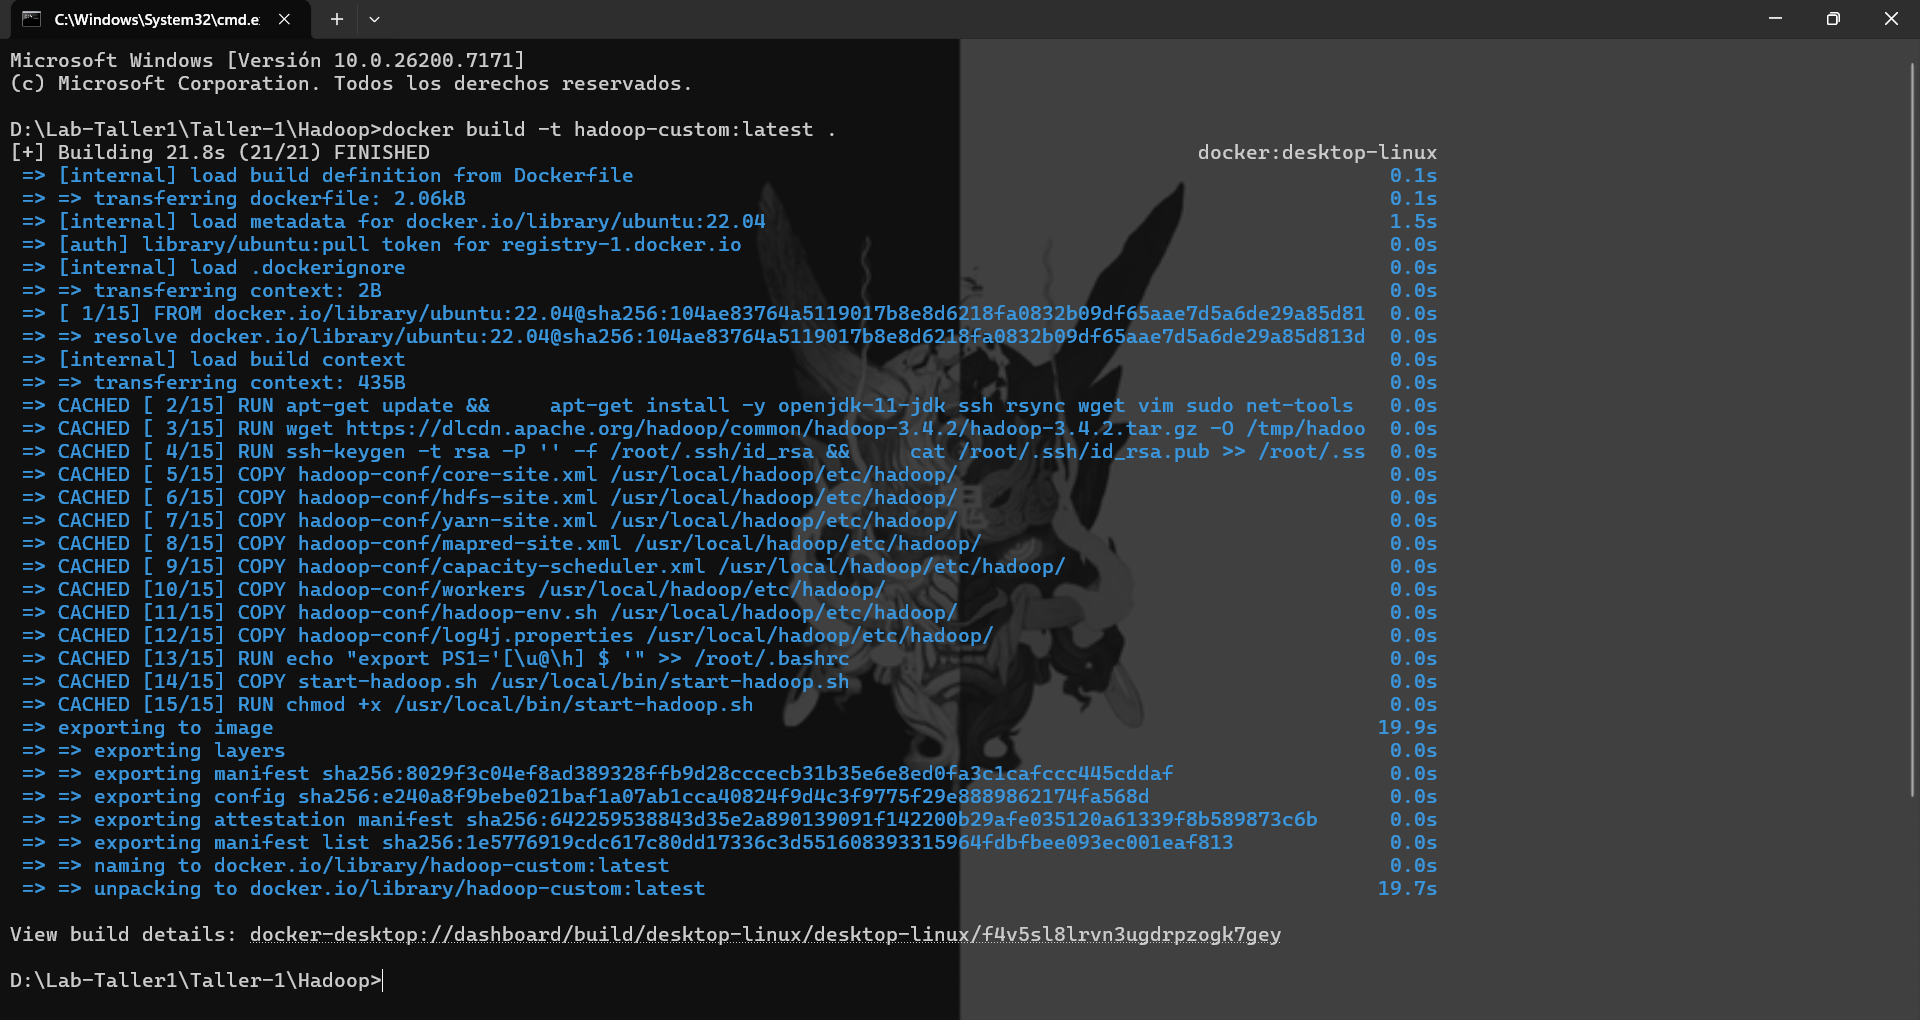
\includegraphics[width=0.95\linewidth]{assets/images/construccion_imagen_Terminal.png}
    \caption{Construcción de la imagen Hadoop desde la terminal.}
    \label{fig:construccion-terminal}
\end{figure}

Asimismo, se verificó la creación de la imagen desde la interfaz gráfica de Docker Desktop (Figura \ref{fig:construccion-dockerGUI}).

\begin{figure}[H]
    \centering
    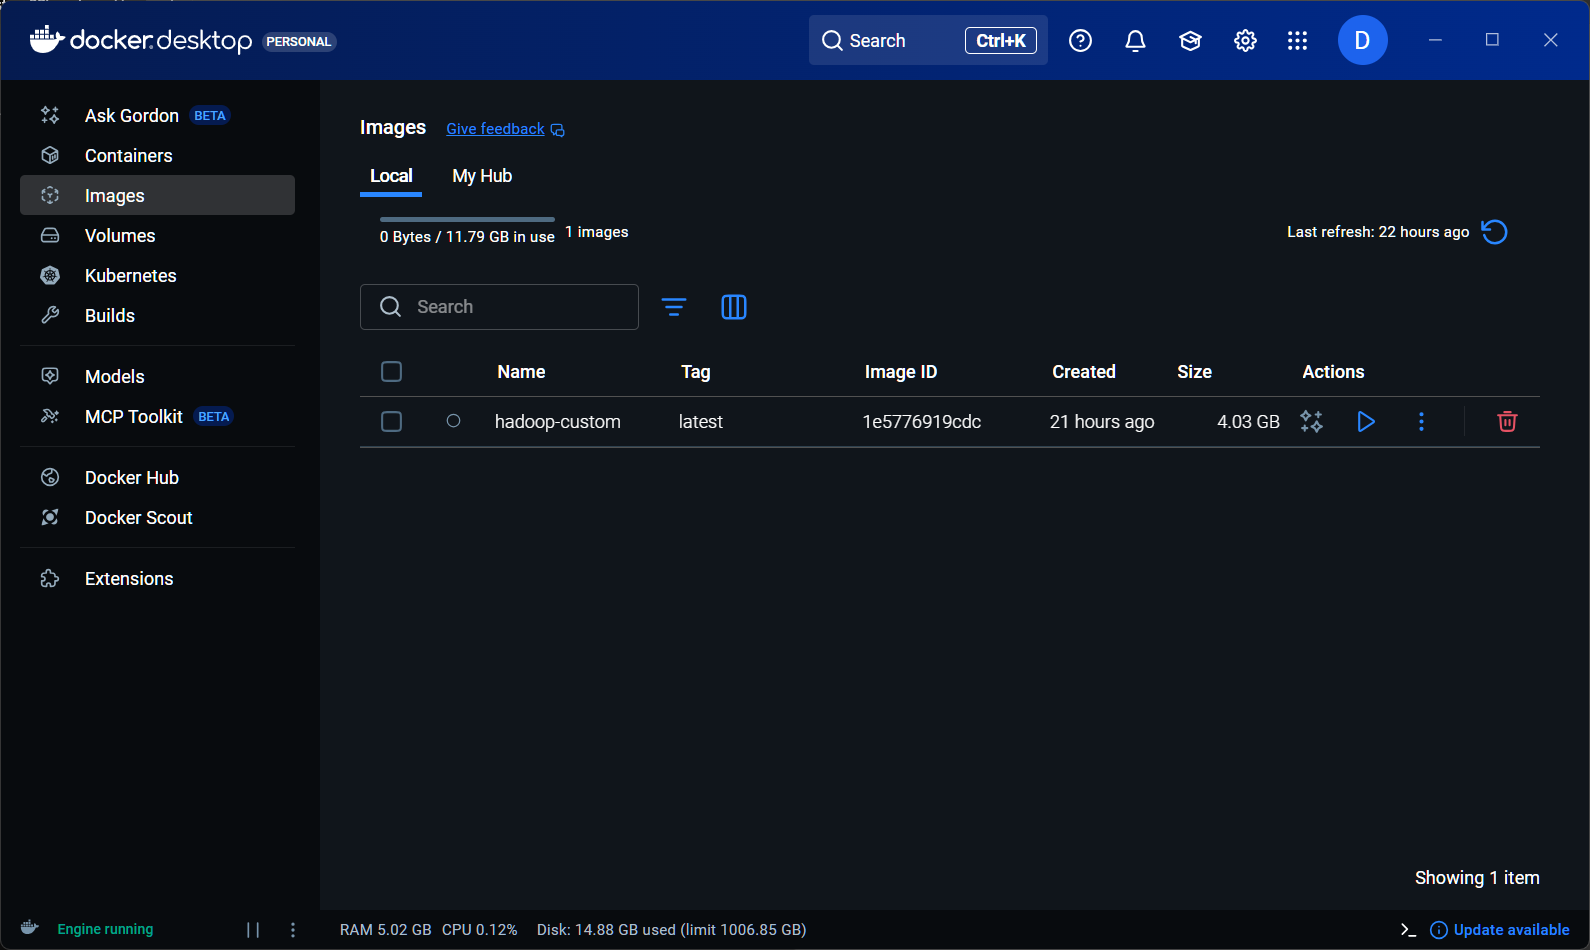
\includegraphics[width=0.95\linewidth]{assets/images/contruccion_imagen_DockerGUI.png}
    \caption{Visualización de la imagen construida en Docker Desktop.}
    \label{fig:construccion-dockerGUI}
\end{figure}

\subsection{Inicio del clúster Hadoop}

Una vez construida la imagen, se procedió al inicio del clúster mediante Docker Compose.

\subsubsection*{Comando ejecutado}
\begin{verbatim}
docker compose up -d
\end{verbatim}

\subsubsection*{Validación del inicio}
La Figura \ref{fig:inicio-contenedores-terminal} muestra el levantamiento exitoso de los contenedores.

\begin{figure}[H]
    \centering
    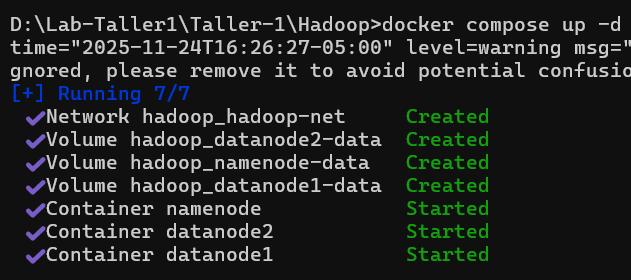
\includegraphics[width=0.95\linewidth]{assets/images/inicio_contenedores_Terminal.png}
    \caption{Levantamiento de contenedores mediante Docker Compose.}
    \label{fig:inicio-contenedores-terminal}
\end{figure}

En Docker Desktop se visualiza el estado de los contenedores activos (Figura \ref{fig:docker-desktop}).

\begin{figure}[H]
    \centering
    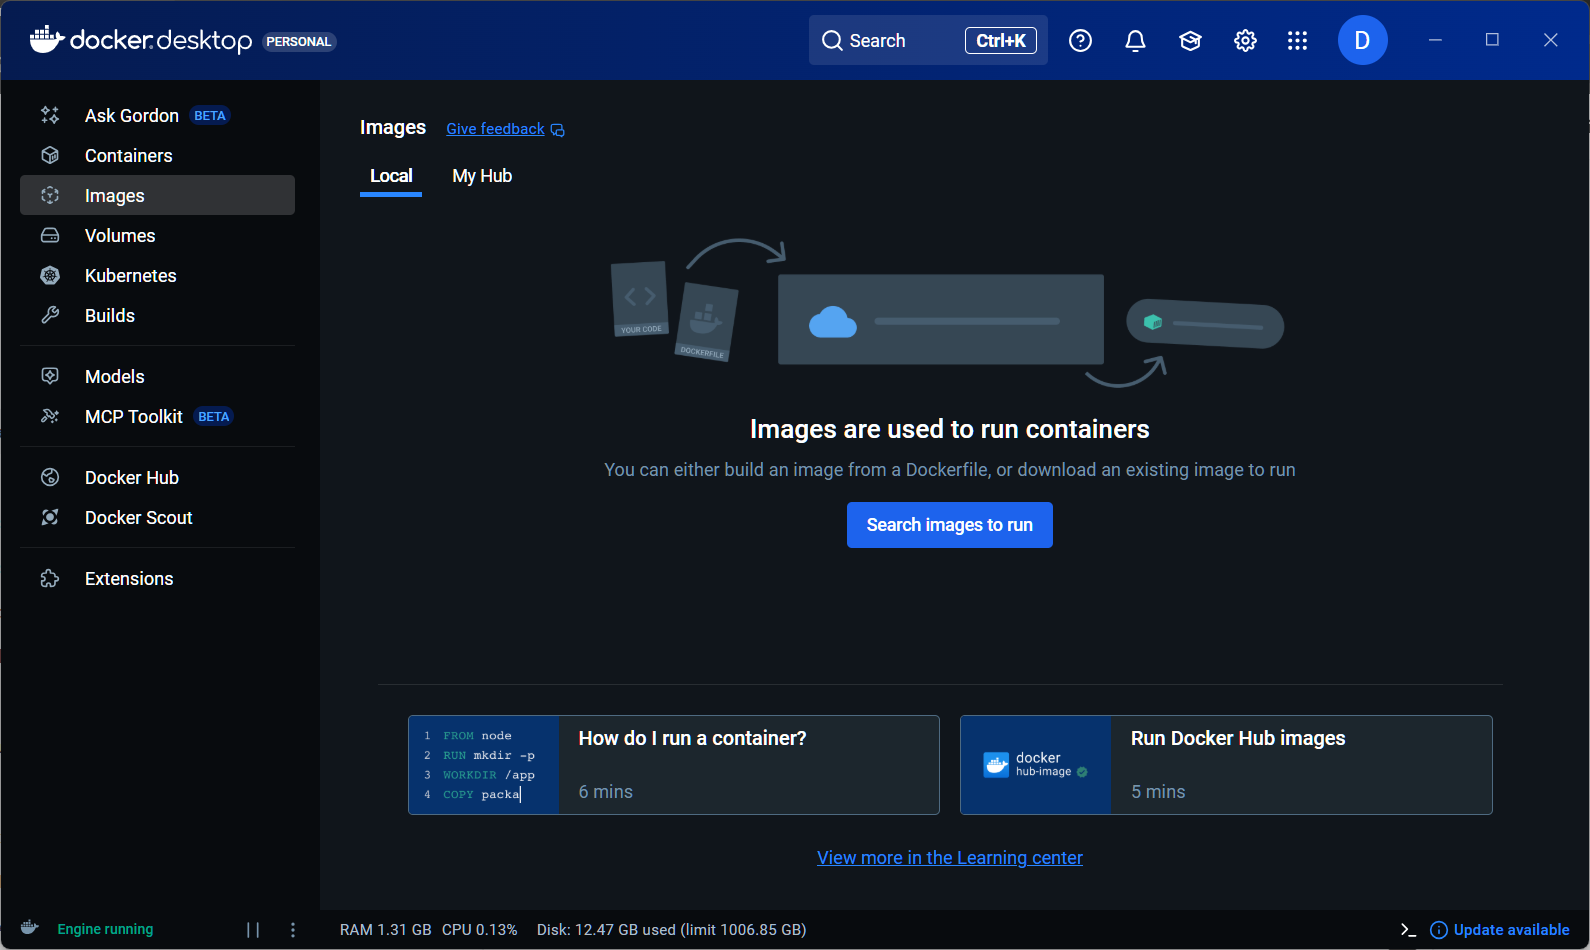
\includegraphics[width=0.95\linewidth]{assets/images/docker_desktop.png}
    \caption{Contenedores activos mostrados en Docker Desktop.}
    \label{fig:docker-desktop}
\end{figure}

\subsubsection*{Verificación del estado}
\begin{verbatim}
docker ps
\end{verbatim}

El estado de los contenedores puede observarse en la Figura \ref{fig:contenedores-status}.

\begin{figure}[H]
    \centering
    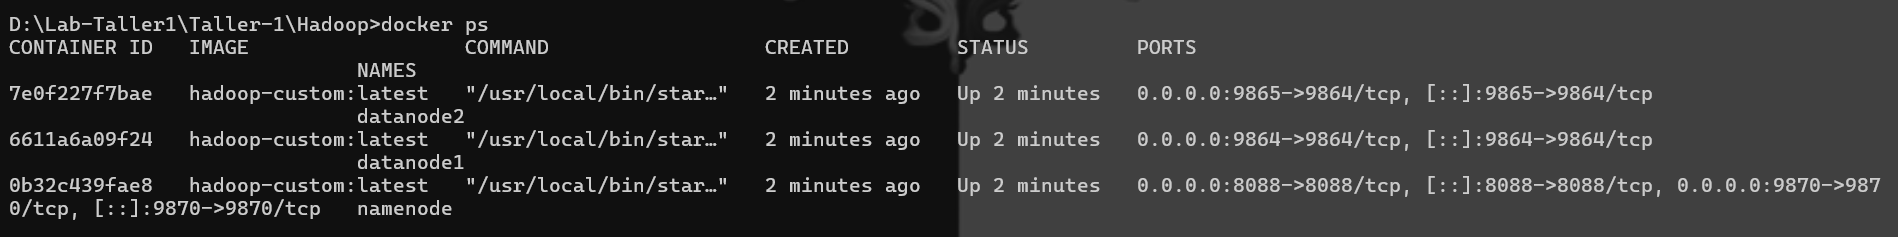
\includegraphics[width=0.95\linewidth]{assets/images/contenedores_status_Terminal.png}
    \caption{Estado de los contenedores Hadoop desde la terminal.}
    \label{fig:contenedores-status}
\end{figure}

\subsection{Acceso al contenedor NameNode}

\subsubsection*{Comando ejecutado}
\begin{verbatim}
docker exec -it namenode bash
\end{verbatim}

Una vez dentro, se verificó la presencia de los procesos principales de Hadoop:

\begin{verbatim}
jps
\end{verbatim}

Las evidencias se presentan en la Figura \ref{fig:servicios-container}.

\begin{figure}[H]
    \centering
    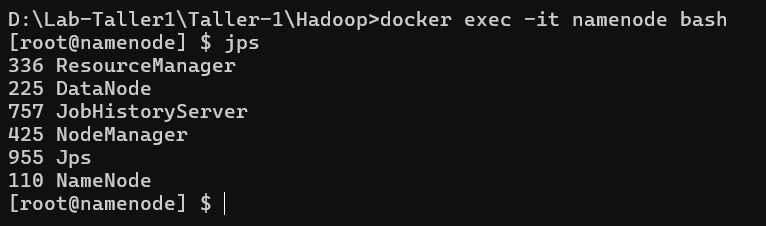
\includegraphics[width=0.95\linewidth]{assets/images/servicios_dentro_del_contenedor_Terminal.png}
    \caption{Procesos ejecutándose en el NameNode.}
    \label{fig:servicios-container}
\end{figure}

\subsection{Verificación del estado de HDFS}

\subsubsection*{Comando ejecutado}
\begin{verbatim}
hdfs dfsadmin -report
\end{verbatim}

Los resultados se dividieron en dos partes según las capturas generadas (Figuras \ref{fig:reporte-hdfs1} y \ref{fig:reporte-hdfs2}).

\begin{figure}[H]
    \centering
    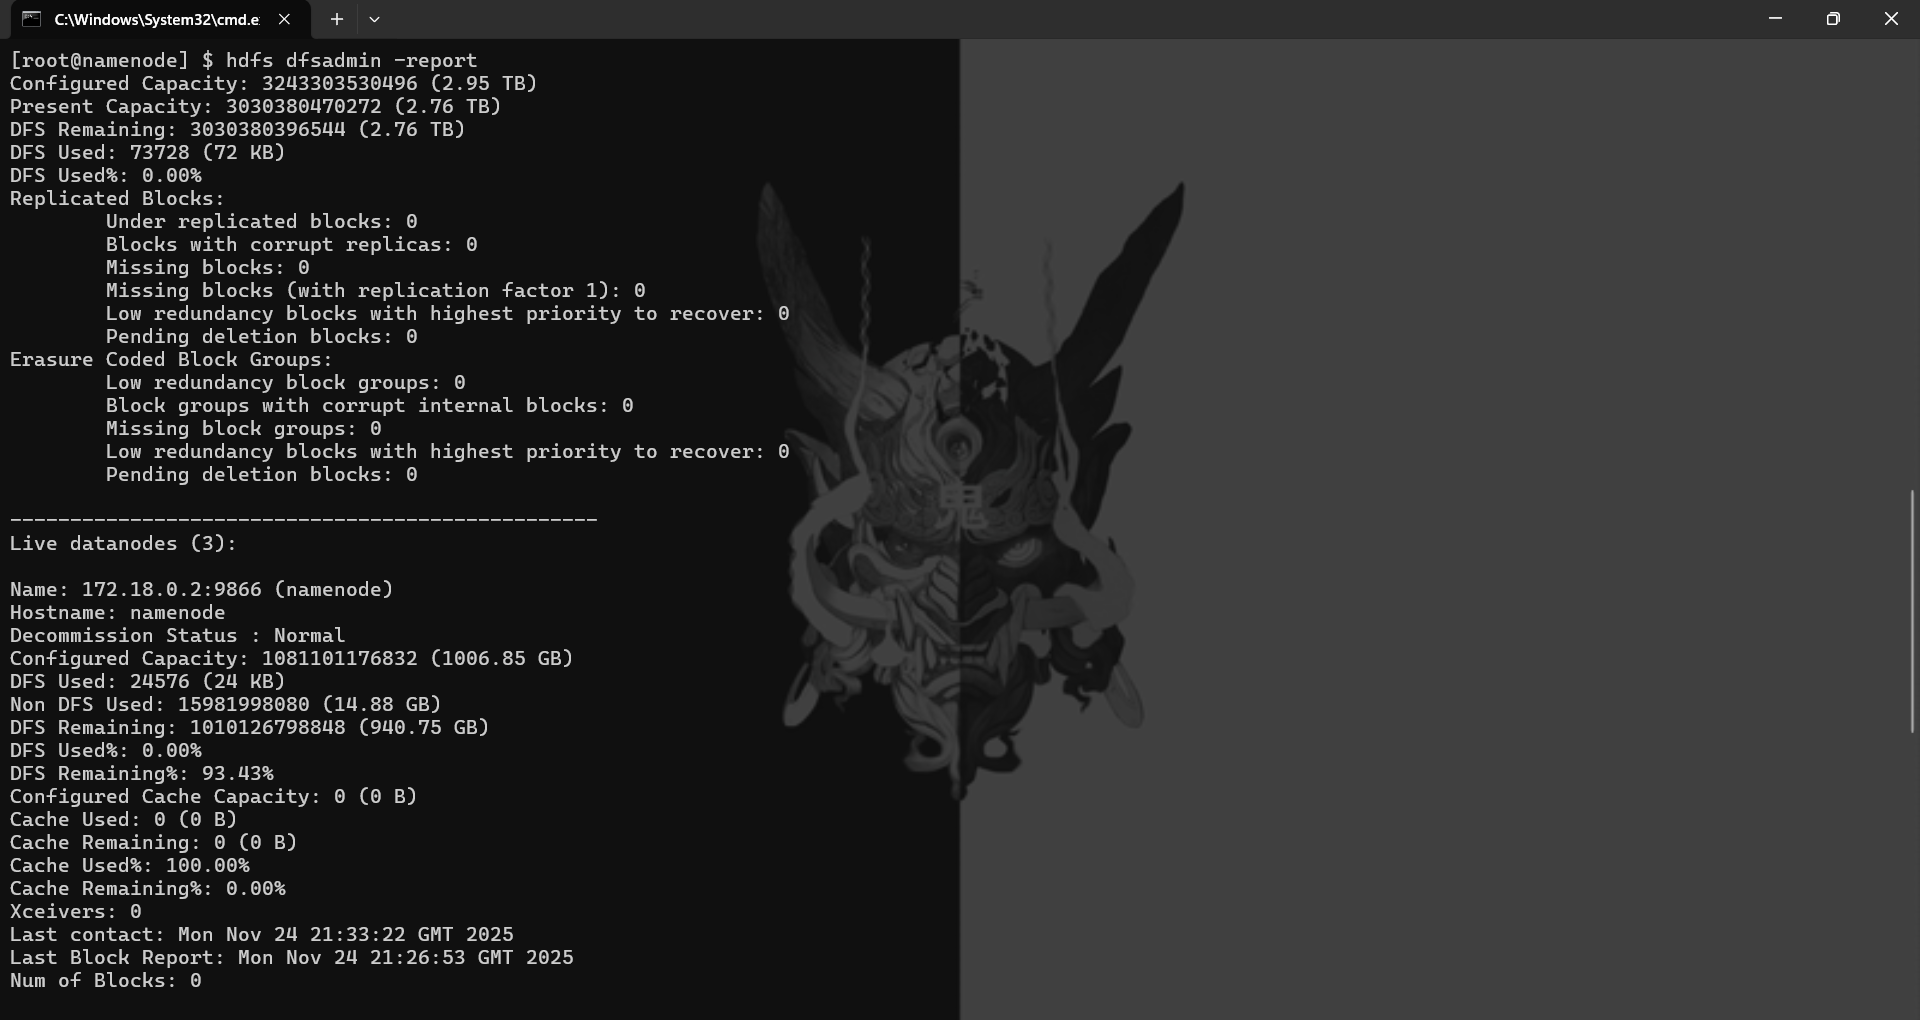
\includegraphics[width=0.95\linewidth]{assets/images/reporte_HDFS_Terminal_part1.png}
    \caption{Reporte general del HDFS (Parte 1).}
    \label{fig:reporte-hdfs1}
\end{figure}

\begin{figure}[H]
    \centering
    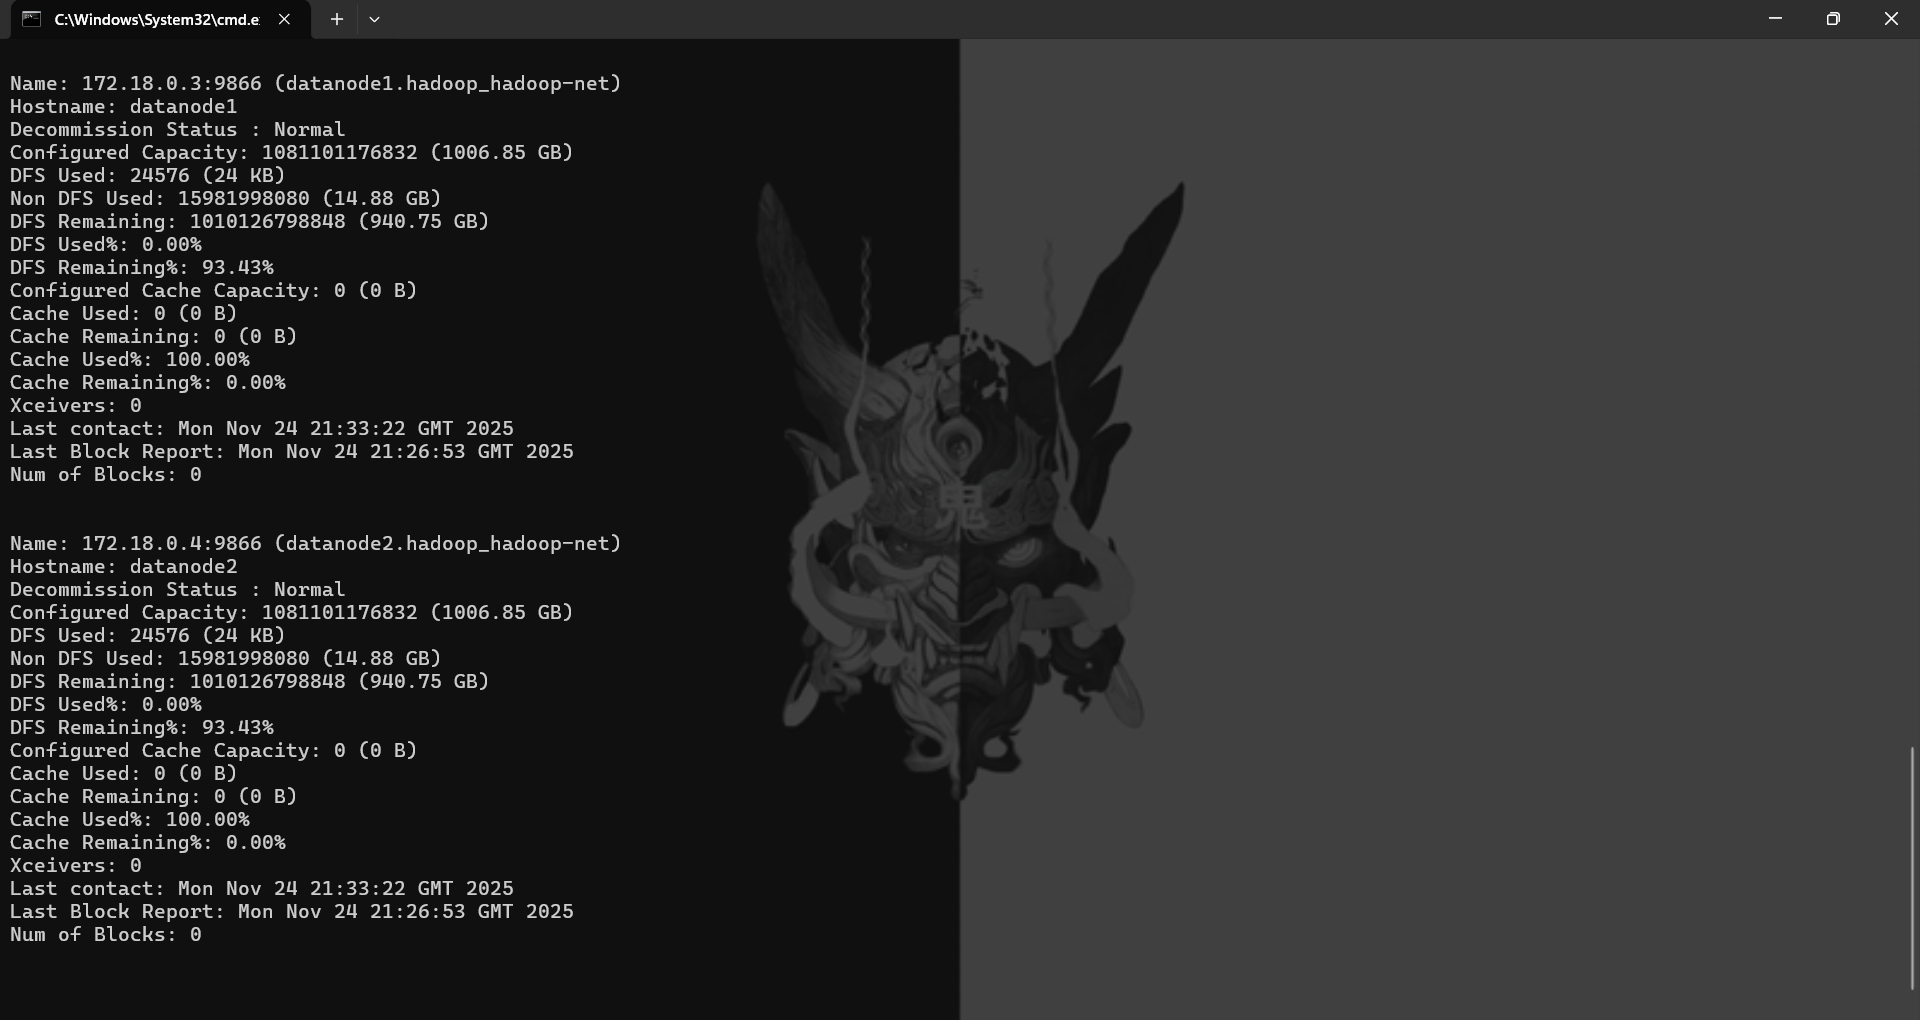
\includegraphics[width=0.95\linewidth]{assets/images/reporte_HDFS_Terminal_part2.png}
    \caption{Reporte general del HDFS (Parte 2).}
    \label{fig:reporte-hdfs2}
\end{figure}

\subsection{Verificación del estado de YARN}

\subsubsection*{Comando ejecutado}
\begin{verbatim}
yarn node -list
\end{verbatim}

El reporte se visualiza en la Figura \ref{fig:nodos-yarn}.

\begin{figure}[H]
    \centering
    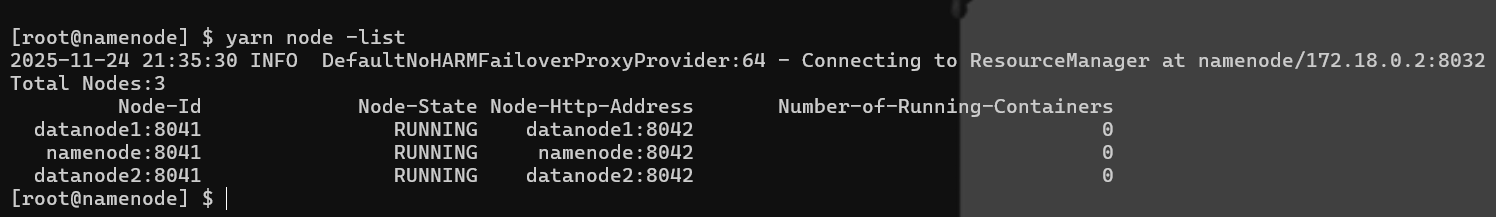
\includegraphics[width=0.95\linewidth]{assets/images/nodos_yarn_Terminal.png}
    \caption{Listado de nodos registrados en YARN.}
    \label{fig:nodos-yarn}
\end{figure}

\subsection{Interfaz Web del NameNode y del ResourceManager}

Las interfaces web permitieron verificar la disponibilidad de los servicios.

\begin{figure}[H]
    \centering
    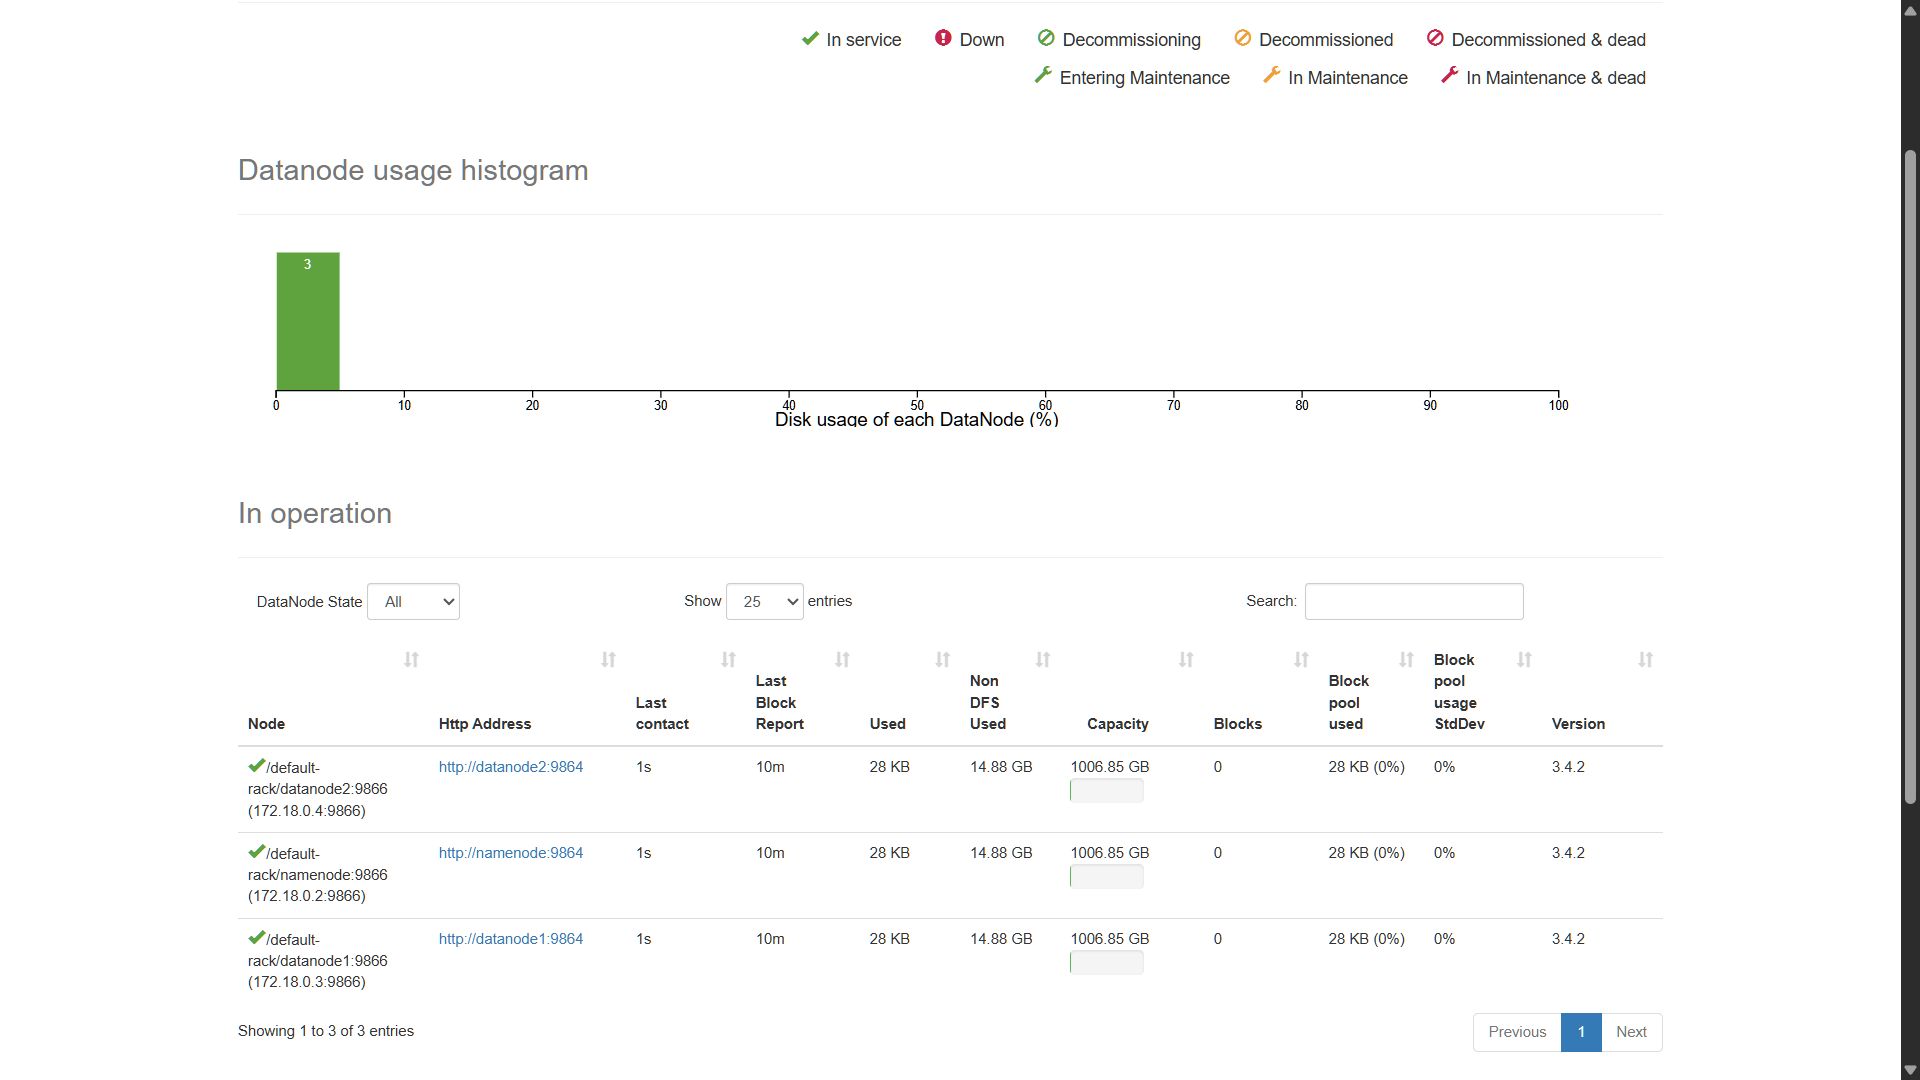
\includegraphics[width=0.95\linewidth]{assets/images/nameNode_Web.png}
    \caption{Interfaz web del NameNode.}
\label{fig:web-namenode}
\end{figure}

\begin{figure}[H]
    \centering
    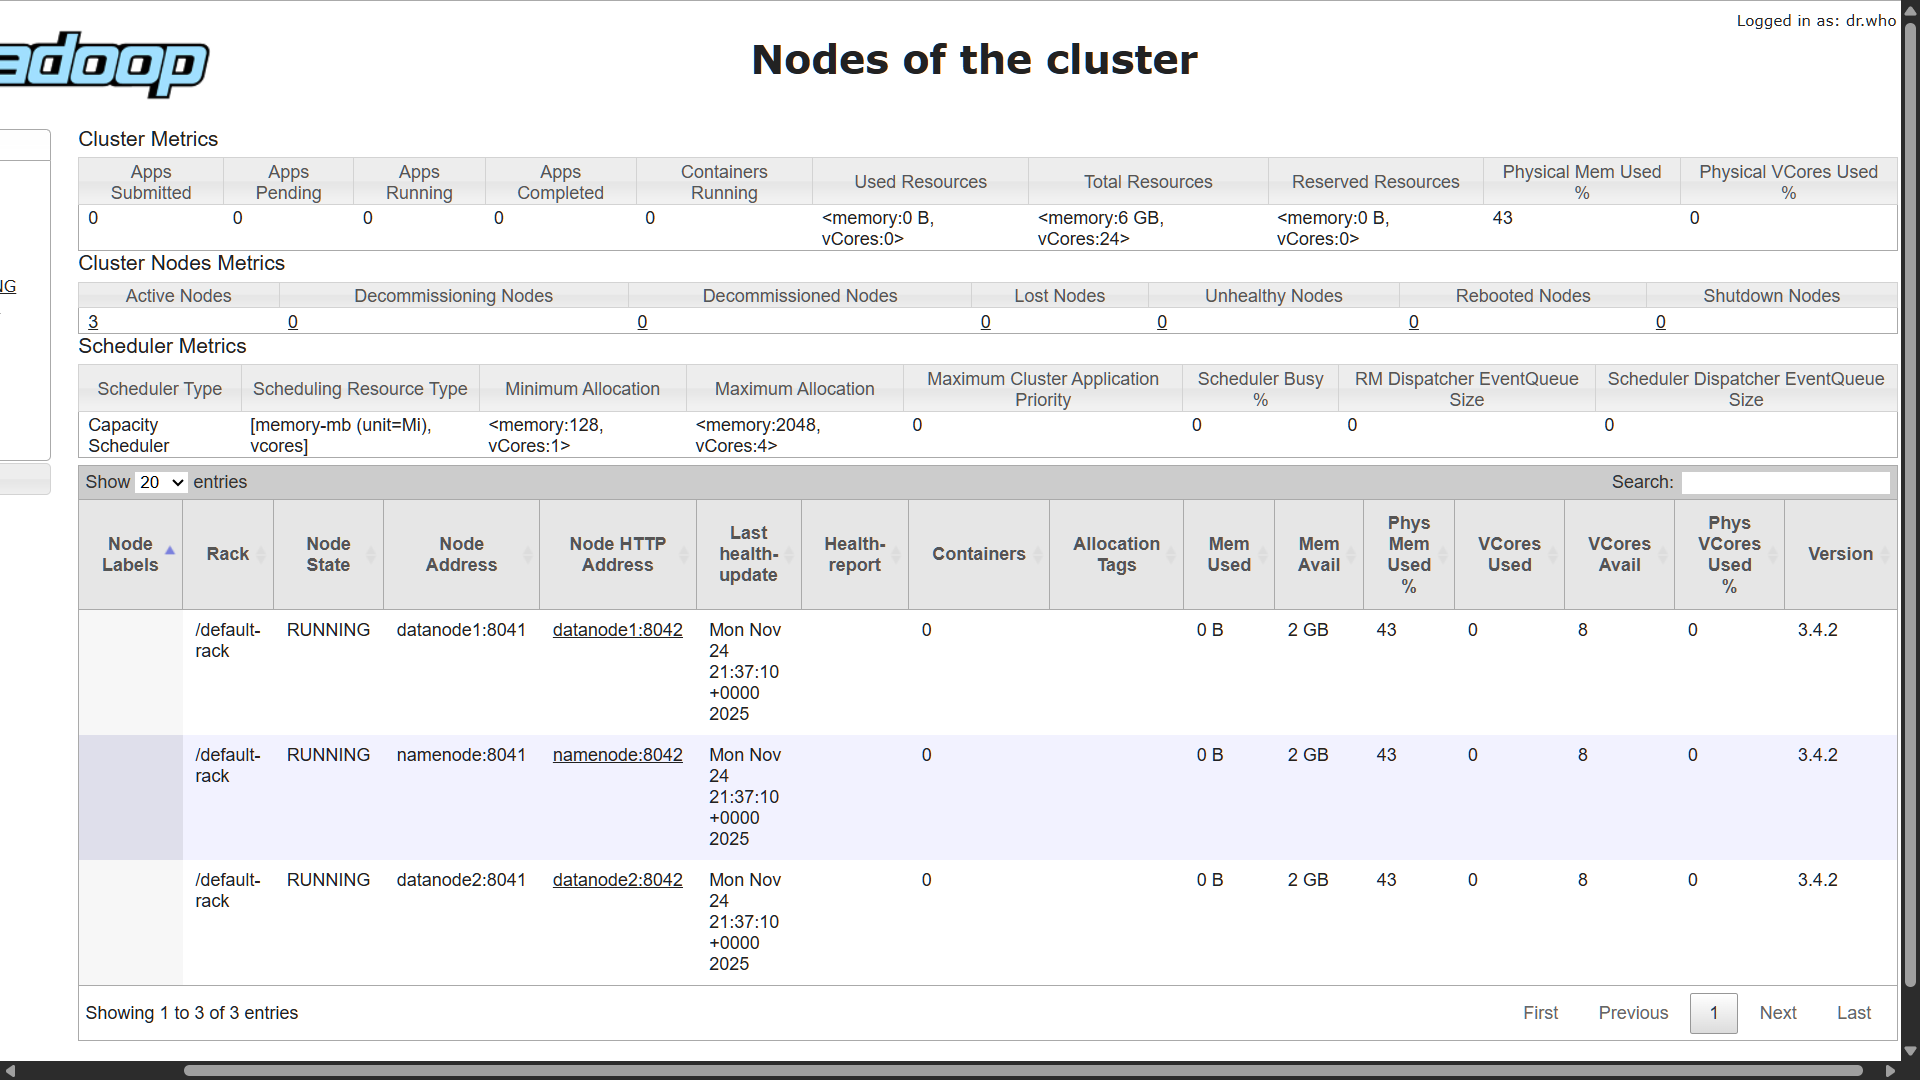
\includegraphics[width=0.95\linewidth]{assets/images/ResourceManager_Web.png}
    \caption{Interfaz web del ResourceManager.}
\label{fig:web-resourcemanager}
\end{figure}

\subsection{Prueba funcional en HDFS y MapReduce}

\subsubsection*{Comandos ejecutados}

Creación de directorios, subida de archivos y lectura:

\begin{verbatim}
hdfs dfs -mkdir /input
echo "Hola Hadoop" > test.txt
hdfs dfs -put test.txt /input
hdfs dfs -ls /input
hdfs dfs -cat /input/test.txt
\end{verbatim}

Generación de archivo masivo:

\begin{verbatim}
for i in {1..100000}; do 
 echo "hadoop mapreduce bigdata analytics \
 processing distributed computing framework";\ 
done > bigfile.txt
\end{verbatim}

La secuencia completa se ilustra en las Figuras \ref{fig:prueba1} y \ref{fig:prueba2}.

\begin{figure}[H]
    \centering
    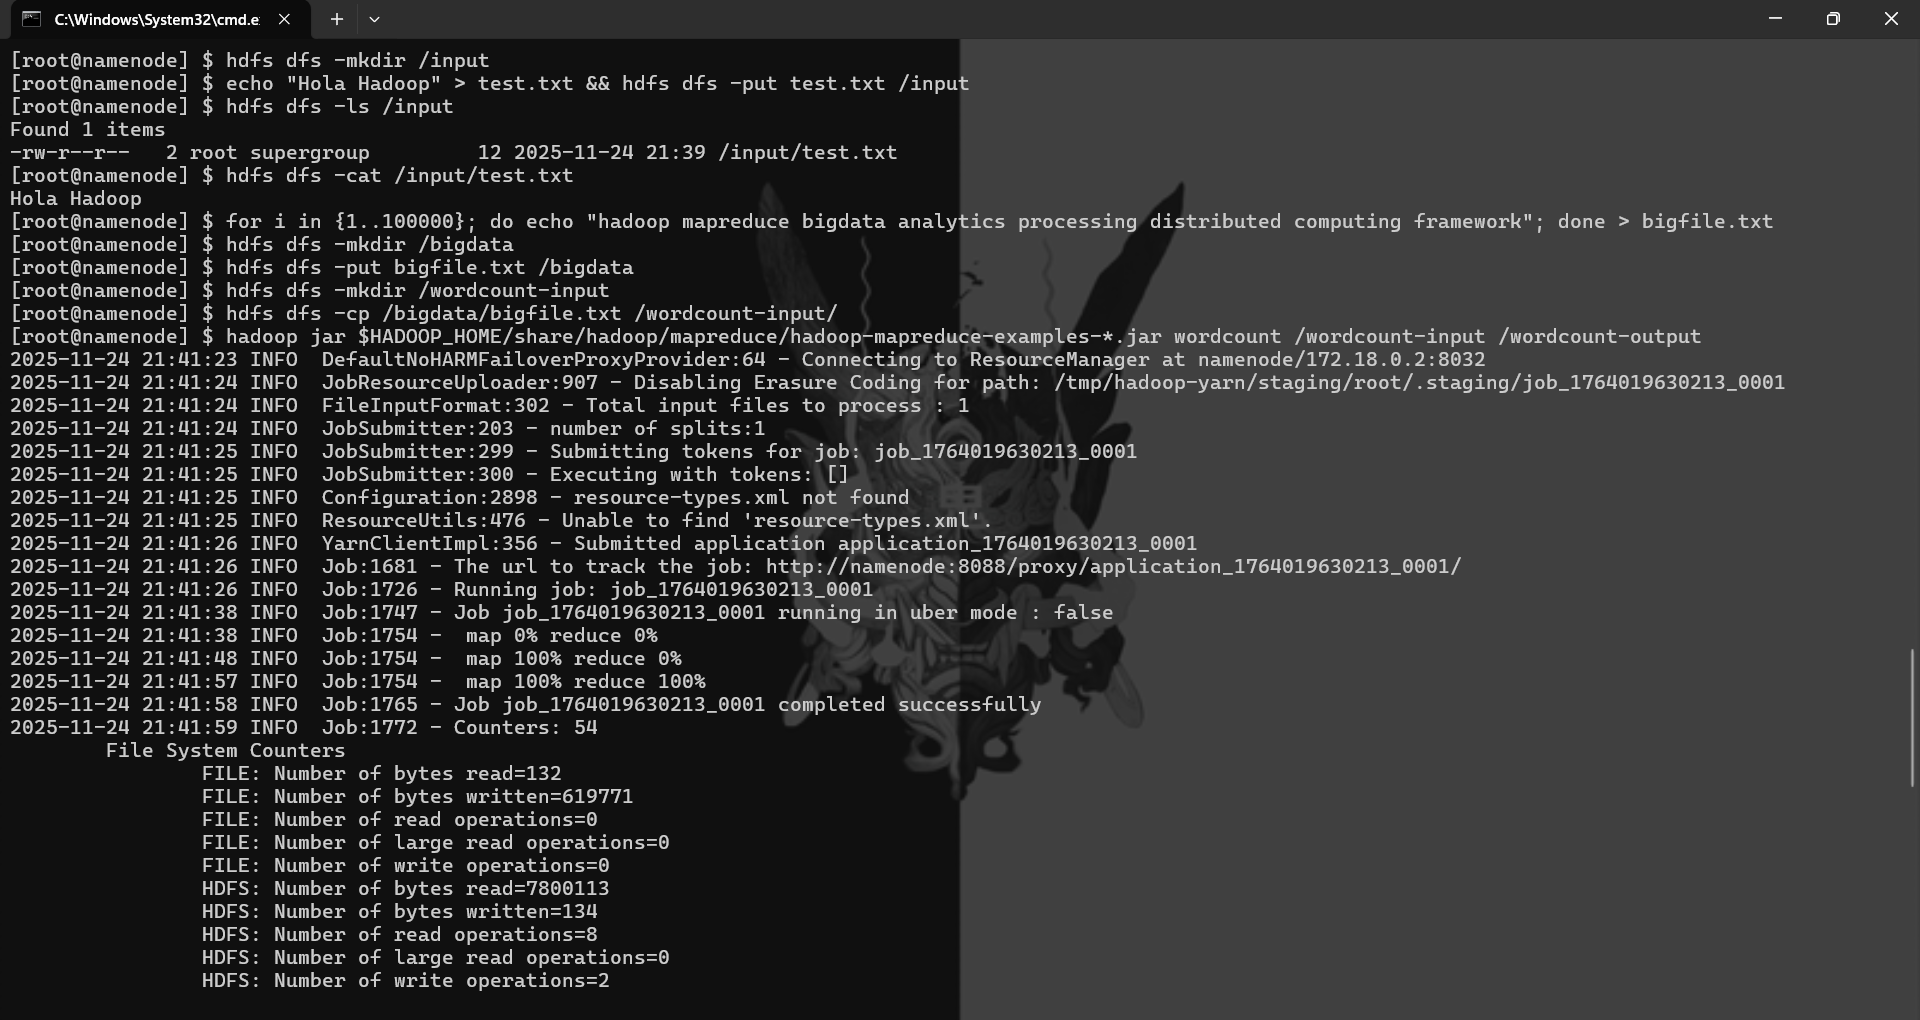
\includegraphics[width=0.95\linewidth]{assets/images/prueba_HDFS_MapReduce_Terminal_part1.png}
    \caption{Ejecución de comandos HDFS y preparación de datos (Parte 1).}
    \label{fig:prueba1}
\end{figure}

\begin{figure}[H]
    \centering
    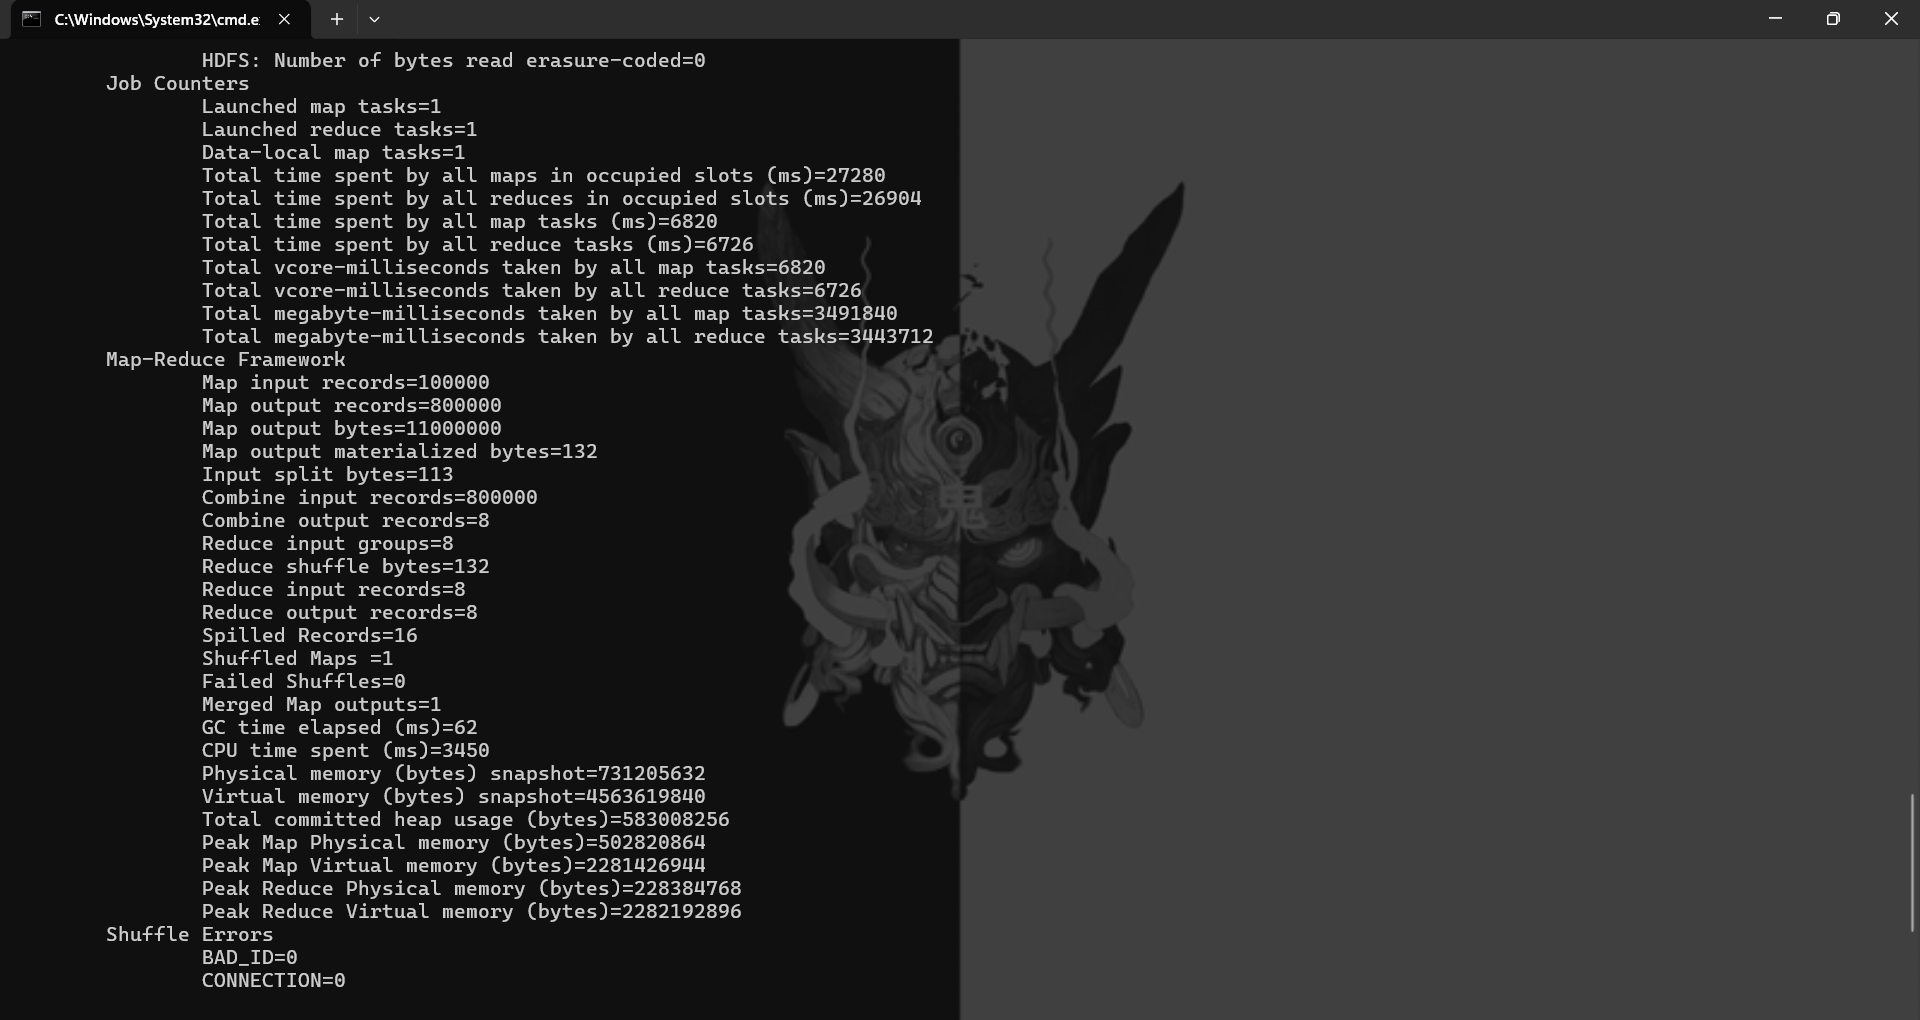
\includegraphics[width=0.95\linewidth]{assets/images/prueba_HDFS_MapReduce_Terminal_part2.png}
    \caption{Ejecución de comandos HDFS y preparación de datos (Parte 2).}
    \label{fig:prueba2}
\end{figure}

\subsubsection*{Ejecución del trabajo WordCount}

\begin{verbatim}
hadoop jar $HADOOP_HOME/share/hadoop/mapreduce/ \
hadoop-mapreduce-examples-*.jar wordcount \
/wordcount-input /wordcount-output
\end{verbatim}

La Figura \ref{fig:estado-mapreduce} muestra el progreso del trabajo.

\begin{figure}[H]
    \centering
    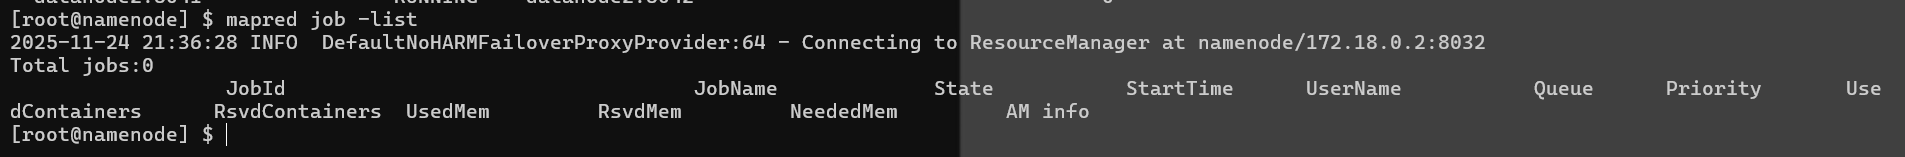
\includegraphics[width=0.95\linewidth]{assets/images/estado_mapReduce_Terminal.png}
    \caption{Ejecución del trabajo MapReduce WordCount.}
    \label{fig:estado-mapreduce}
\end{figure}

\subsubsection*{Resultados generados}

\begin{verbatim}
hdfs dfs -cat /wordcount-output/part-r-00000 | head -20
\end{verbatim}

Los resultados pueden visualizarse en la Figura \ref{fig:resultados-mapreduce}.

\begin{figure}[H]
    \centering
    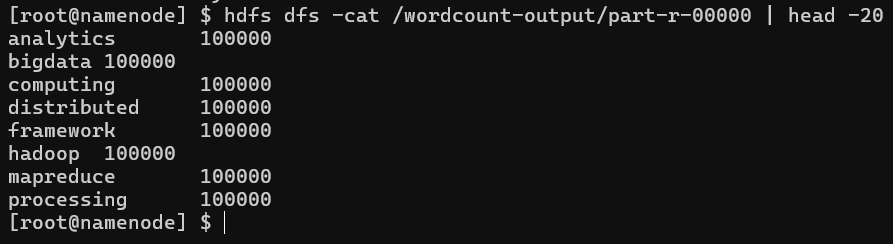
\includegraphics[width=0.95\linewidth]{assets/images/resultados_MapReduce_Terminal.png}
    \caption{Resultados del trabajo WordCount.}
    \label{fig:resultados-mapreduce}
\end{figure}

\subsection{Problemas Encontrados y Soluciones Aplicadas}

Durante el desarrollo del laboratorio se identificaron diversos problemas técnicos que afectaron la correcta inicialización y operación del clúster Hadoop ejecutado sobre contenedores Docker. A continuación, se presenta un análisis exhaustivo de los errores detectados, sus causas raíz y las soluciones implementadas. Este apartado constituye una referencia integral del proceso de depuración efectuado, evidenciando la complejidad inherente a la configuración distribuida de Hadoop en entornos virtualizados.

\subsubsection*{1. Inconsistencias en el formateo del NameNode}

Uno de los primeros inconvenientes observados se relacionó con el uso incorrecto del comando \texttt{hdfs namenode -format}, el cual fue ejecutado cuando los servicios de Hadoop ya se encontraban activos dentro de los contenedores. Este procedimiento generó conflictos entre el \textit{clusterID} del NameNode y los DataNodes, impidiendo que estos últimos pudieran registrarse correctamente.

\textbf{Solución:} se estableció un flujo de inicialización adecuado, donde el formateo del NameNode se realiza \textit{antes} del inicio de cualquier servicio Hadoop y únicamente una vez por ciclo de creación del entorno. Además, se empleó \texttt{docker compose down -v} para garantizar la eliminación completa de volúmenes previos.

\subsubsection*{2. Ejecución anticipada de servicios Hadoop mediante scripts}

El script \texttt{start-hadoop.sh} incluía inicialmente instrucciones para iniciar automáticamente los procesos de Hadoop (NameNode, DataNode, ResourceManager y NodeManager) al iniciar los contenedores. Esta ejecución prematura provocó que los DataNodes intentaran establecer conexión con un NameNode aún no formateado, generando estados inconsistentes.

\textbf{Solución:} se modificó el script para eliminar cualquier comando de inicio automático de Hadoop, permitiendo un control manual y secuencial del proceso de arranque.

\subsubsection*{3. Falta del archivo de configuración \texttt{capacity-scheduler.xml}}

El servicio YARN, específicamente el \textit{ResourceManager}, fallaba durante la inicialización con el error:

\begin{verbatim}
java.lang.IllegalStateException: Queue configuration missing child /
queue names for root
\end{verbatim}

Este error se debía a la ausencia del archivo \texttt{capacity-scheduler.xml}, indispensable para definir las colas del planificador de capacidad.

\textbf{Solución:} se generó un archivo \texttt{capacity-scheduler.xml} válido, con la definición básica de la cola \texttt{default}, y posteriormente se añadió la instrucción correspondiente en el \texttt{Dockerfile} para copiarlo en la ruta correcta.

\subsubsection*{4. Errores en el \texttt{Dockerfile} al intentar reescribir scripts internos}

Durante la reconfiguración del entorno, se intentó reescribir el script \texttt{start-hadoop.sh} desde el \texttt{Dockerfile} utilizando múltiples comandos \texttt{RUN echo}. Sin embargo, el uso incorrecto de comillas internas generó errores de parseo del Dockerfile, ocasionando fallos al construir la imagen.

\textbf{Solución:} se optó por mantener el script como archivo externo dentro del directorio del proyecto y utilizar una sola instrucción \texttt{COPY} en el Dockerfile para garantizar su transferencia íntegra al contenedor.

\subsubsection*{5. Desajustes entre las rutas reales del sistema y las definidas en HDFS}

Se detectaron múltiples discrepancias entre las rutas configuradas en \texttt{hdfs-site.xml} y las rutas efectivamente creadas dentro de los contenedores. Por ejemplo, Hadoop esperaba almacenar los bloques en:

\begin{verbatim}
file:///usr/local/hadoop/data/dfs/datanode
\end{verbatim}

mientras que, en la práctica, se habían creado rutas alternativas como \texttt{/usr/local
/hadoop/data/dfs/datanode2}.

\textbf{Solución:} se unificaron todas las rutas, creando únicamente los directorios específicamente definidos en los archivos de configuración, asegurando así la coherencia entre el sistema de archivos del contenedor y las rutas esperadas por Hadoop.

\subsubsection*{6. Registro fallido de los DataNodes en el NameNode}

A pesar de que los DataNodes indicaban estar ejecutándose (comprobado con el comando \texttt{jps}), el NameNode reportaba:

\begin{verbatim}
Live datanodes: 0
Configured Capacity: 0
\end{verbatim}

Este comportamiento se debía a inconsistencias previas en volúmenes, permisos, rutas erróneas y conflictos de \textit{clusterID}.

\textbf{Solución:} tras limpiar completamente los volúmenes, corregir rutas y restablecer el flujo de inicialización, los DataNodes lograron registrarse correctamente.

\subsubsection*{7. Problemas de conexión con el ResourceManager}

En varias ocasiones, el comando:

\begin{verbatim}
yarn node -list
\end{verbatim}

permanecía en espera indefinida debido a que el ResourceManager aún no estaba disponible o no había iniciado correctamente.

\textbf{Solución:} se implementó un periodo de espera mayor en el script de arranque para permitir la inicialización completa de YARN, especialmente cuando los recursos del sistema anfitrión son limitados.

\subsubsection*{8. Fallos al ejecutar trabajos MapReduce debido a entradas inexistentes}

Inicialmente, se ejecutaron pruebas de MapReduce sin haber cargado archivos de entrada en HDFS, lo que generó salidas vacías o errores del tipo:

\begin{verbatim}
FileAlreadyExistsException
\end{verbatim}

o mensajes indicando ausencia de datos de entrada.

\textbf{Solución:} se estructuró un flujo correcto donde primero se genera y carga un archivo (por ejemplo, \texttt{bigfile.txt}) en el directorio \texttt{/wordcount-input}, y posteriormente se ejecuta el trabajo MapReduce. Asimismo, se eliminó sistemáticamente el directorio de salida previo para evitar conflictos.

\subsubsection*{9. Problemas de permisos y creación automática de directorios}

En diversos registros se mostraban advertencias como:

\begin{verbatim}
WARNING: /usr/local/hadoop/logs does not exist. Creating.
\end{verbatim}

indicando que algunos directorios no se encontraban creados o presentaban permisos insuficientes para Hadoop.

\textbf{Solución:} se estandarizó la creación de directorios en el Dockerfile y se asignaron los permisos adecuados dentro del contenedor.

\subsubsection*{10. Falta de sincronización entre servicios dentro de los contenedores}

Finalmente, se identificó que algunos servicios de Hadoop iniciaban antes de que otros estuvieran completamente activos, lo que provocaba errores de conexión tanto en HDFS como en YARN.

\textbf{Solución:} se reestructuraron los tiempos de espera en \texttt{start-hadoop.sh} y se adoptaron procesos de validación secuencial para garantizar que cada servicio estuviera operativo antes de avanzar con el siguiente componente.

\bigskip

Luego de haber solucionado se presentaron problemas mínimos que no afectan como tal a la funcionamiento principal ni mucho menos a los objetivos del taller los cuales se los presenta a continuación siguientes:

\begin{itemize}
    \item \textbf{Tiempos prolongados de inicialización de YARN}.  
    \textit{Solución:} esperar entre 2 y 3 minutos antes de ejecutar comandos administrativos.

    \item \textbf{Advertencia de atributo obsoleto \texttt{version} en Docker Compose.}  
    \textit{Solución:} se mantuvo la compatibilidad evitando modificar el archivo, dado que no afecta la ejecución.

    \item \textbf{Demoras en la interfaz web del ResourceManager.}  
    \textit{Solución:} revisar capacidad de memoria disponible en el sistema anfitrión.

    \item \textbf{Posible lentitud al generar archivos grandes mediante \texttt{for}.}  
    \textit{Solución:} uso de redirección directa a un archivo con líneas repetitivas, optimizando su generación.
\end{itemize}

En conjunto, la resolución de estos problemas permitió estabilizar el entorno distribuido y garantizar un funcionamiento óptimo del clúster de Hadoop sobre Docker, demostrando la importancia de un control riguroso de rutas, tiempos de inicialización, consistencia entre volúmenes y congruencia entre archivos de configuración.